% !TeX program = lualatex
\documentclass[a4paper,12pt,twoside]{article}
\usepackage{hot_report}
\usepackage[utf8]{inputenc}

\title{Displaced Persons Head Counts}
\author{Sara Amadi, Asha Mustapher, Johanes Petro, Barnabas Caro, Ivan Gayton }
\date{July 2019}

\begin{document}

\maketitle


\renewcommand{\baselinestretch}{1.5}\normalsize %the number controls the spacing between ToC lines
\tableofcontents
\renewcommand{\baselinestretch}{1.0}\normalsize

\newpage

\section{Introduction}
\begin{multicols}{2}
MSF often needs to know the number of displaced people in a camp, settlement, Protection of Civilians area, or other context. Population numbers are useful to prioritize contexts where there aren't enough resources to respond to all of the calls for help. They can facilitate rational HR and supply planning, and inform advocacy in cases where other actors are not taking their responsibilities to meet the needs of the population (as with inadequate food distributions). 

"Head counts" are notoriously difficult to perform accurately, safely, and ethically. They can be fraught with economic incentives---people and agencies often attempt to exaggerate numbers to attract funding---and political sensitivities. Governments, in an attempt to deny the existence of problems in their territory, may attempt to pressure agencies to under-count displaced persons. Some methods of counting people are coercive and dangerous---for example people may be forced into barbed-wire enclosures for counting purposes---and MSF will not wish to participate in such activities despite needing accurate population figures. 

We have looked at a number of settings where head counts are needed, and asked
those intervening what population information they need, what they actually have, the shortcomings of that information, and how they currently address it. We are now proposing several potential methods to improve upon the status quo. These are informed by the information we have gathered here as well as our work with the Missing Maps project.

Our recommendations include relatively novel techniques such as drone surveys and mobile data collection using unskilled community members. These are not intended to be prescriptive or exhaustive, but rather to point the way toward several possible pilot projects. Additionally, we discuss the many ethical, practical, and security-related limitations of these methods, and propose a basic framework to assess the appropriateness of various head count methods.

\end{multicols}

\section{Context and Need Typology}
\begin{multicols}{2}
Before deciding to do a head count---and choosing a method---first assess what population data is available, why you need the population figures, and what exact information you need. 

For example, in the case of a large, rapid displacement (hundreds of thousands of people arriving in an unprepared camp site), it's likely that the immediate need will be a very rough count---just sufficient to order a sensible number of plastic sheets, jerry cans, vaccine doses, and food with introduction of geographic data for potential sites to intervene on.

In other cases, for example, a long-established camp setting, improving medical quality and ensuring the most vulnerable receive care may require detailed information from each household or a considerable sample size---number of children, vulnerable members, pregnant women, and so forth. The choice of tools should follow from the needs.

\end{multicols}

\newpage
At the risk of oversimplifying, we have chosen three broad categories of need for population counts:
\begin{itemize}
    \item Rapid household count (usually counting tents or structures)
    \item Rapid household survey (counting the residents of each structure or a sample subset thereof)
    \item Detailed household survey (enumerating the residents of structures, including demographic information)
\end{itemize}

\subsection{Rapid Household Count}
 This does not enumerate all residents, but only counts the households, typically by using tents or other structures as a proxy for the number of people. We usually do not visit each structure, but simply estimate the number of structures and multiply by an expected number of people per structure.

\noindent
\textbf{Examples of use-cases:}

\begin{itemize}
  \item Recent displacement
  \item To estimate the resources needed for blanket distributions
  \item To compare and prioritize needs between several potential interventions
\end{itemize}

\noindent
\textbf{Possible Methods:}

\begin{itemize}
  \item From above
  \begin{itemize}
    \item Satellite
    \item Aircraft (plane or helicopter)
    \item Drone (fixed-wing or multicopter)
    \item Balloon or kite
  \end{itemize}
\end{itemize}

\begin{itemize}
  \item From the ground
  \begin{itemize}
    \item GPS survey to get total area, multiply by structure density and persons/structure
    \item Count rows and columns, multiply for structure count
  \end{itemize}
\end{itemize}

\noindent
\textbf{Completion time: 1-3 days}

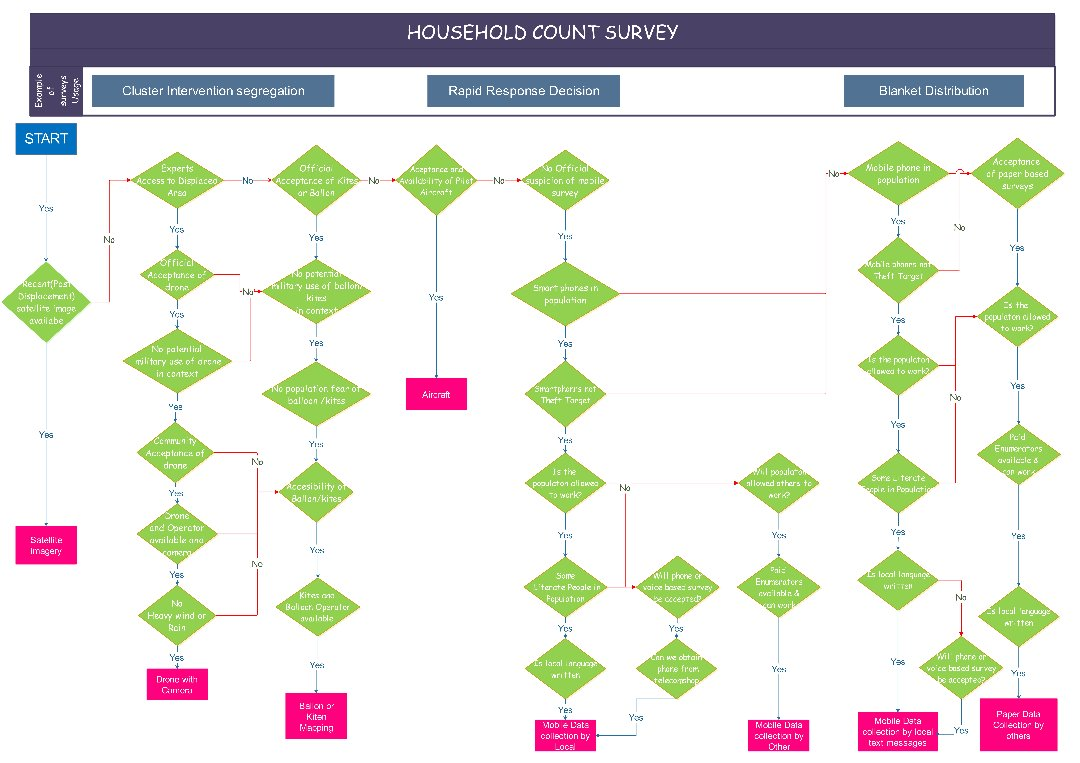
\includegraphics[width=1\textwidth]{images/Household_Count.jpeg}

\newpage
\subsection{Rapid Household Survey}
This method provides more detail on the demographics of the population, typically at least the number of men, women, and children. Here we visit each structure and speak to the residents, but gather only basic information (number of people disaggregated by age and sex) for each household. This very simple data can usually be collected quickly with relatively low-skilled enumerators.

\noindent
\textbf{Examples of use-cases:}

\begin{itemize}
    \item To conduct a basic needs assessment for a given population (i.e. ordering supplies)
    \item To determine the extent and distribution of primary health care needed for patients
\end{itemize}

\noindent
\textbf{Possible Methods:}
\begin{itemize}
    \item Mobile Data Collection
    \item Paper-based surveys
    \item Aggregate medical records and "denominator tool" calculations
    \item Spatial sampling with a subset of households surveyed
\end{itemize}

\noindent
\textbf{Completion time:} 1-2 weeks

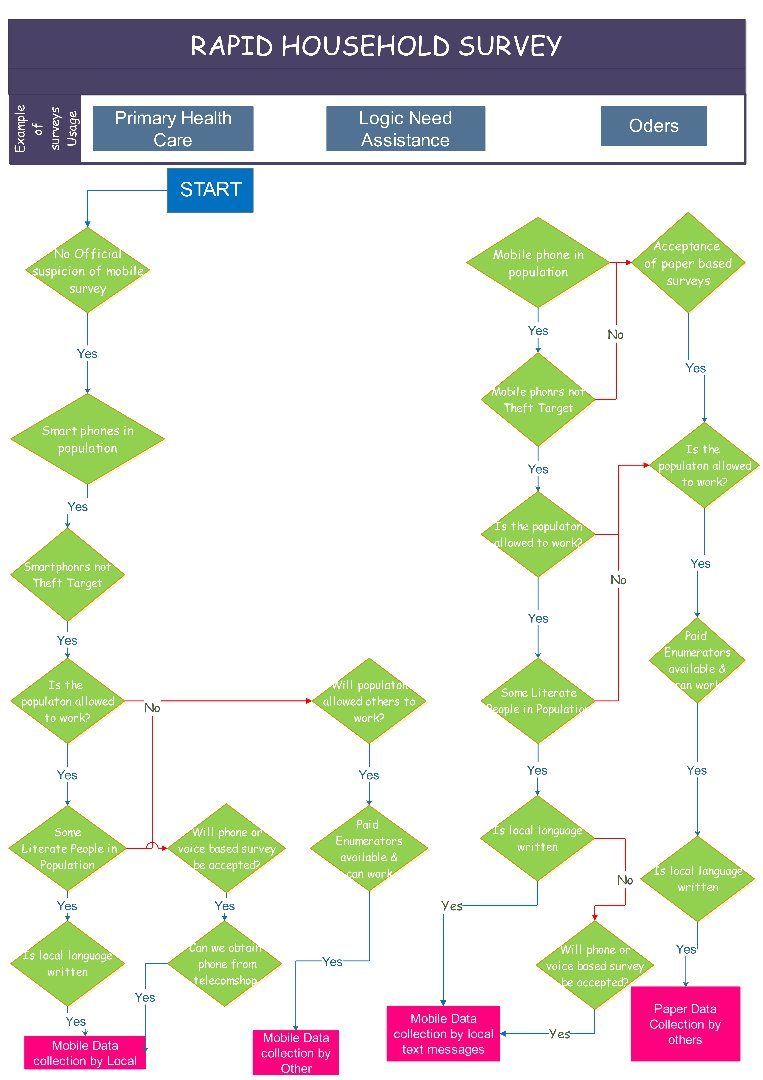
\includegraphics[width=0.9\textwidth]{images/Rapid_Household_Survey.jpeg}

\subsection{Detailed Household Survey}
Sometimes you need to understand the demographics, vulnerability, and specific characteristics of people within each household. In this case you will conduct an extensive survey at each household (though this may be not be every household---it may be a subset chosen as a sample from which to extrapolate the characteristics of the whole population). 



\noindent
\textbf{Examples of use-cases:}
\begin{itemize}
    \item Established camp where we feel that some people do not have access to care and may not be presenting in clinics
    \item Setting where a subset of the population is unusually vulnerable, such as malnourished children, HIV/TB-positive people, etc
    \item Setting with seemingly unexplained mortality
    \item Setting where MSF needs to advocate on behalf of a specific segment of the population (i.e. women lacking access to safe firewood collection) and wishes to have concrete numbers with which to call for others to take their responsibilities
\end{itemize}

\noindent
\textbf{Possible Methods:}
\begin{itemize}
    \item Mobile Data Collection
    \item Paper-based surveys
    \item Spatial sampling with a subset of households surveyed
    \item Integration of mobile data collection into Community Health Worker and outreach practice
\end{itemize}

\noindent
\textbf{Completion time: 1 month to ongoing}

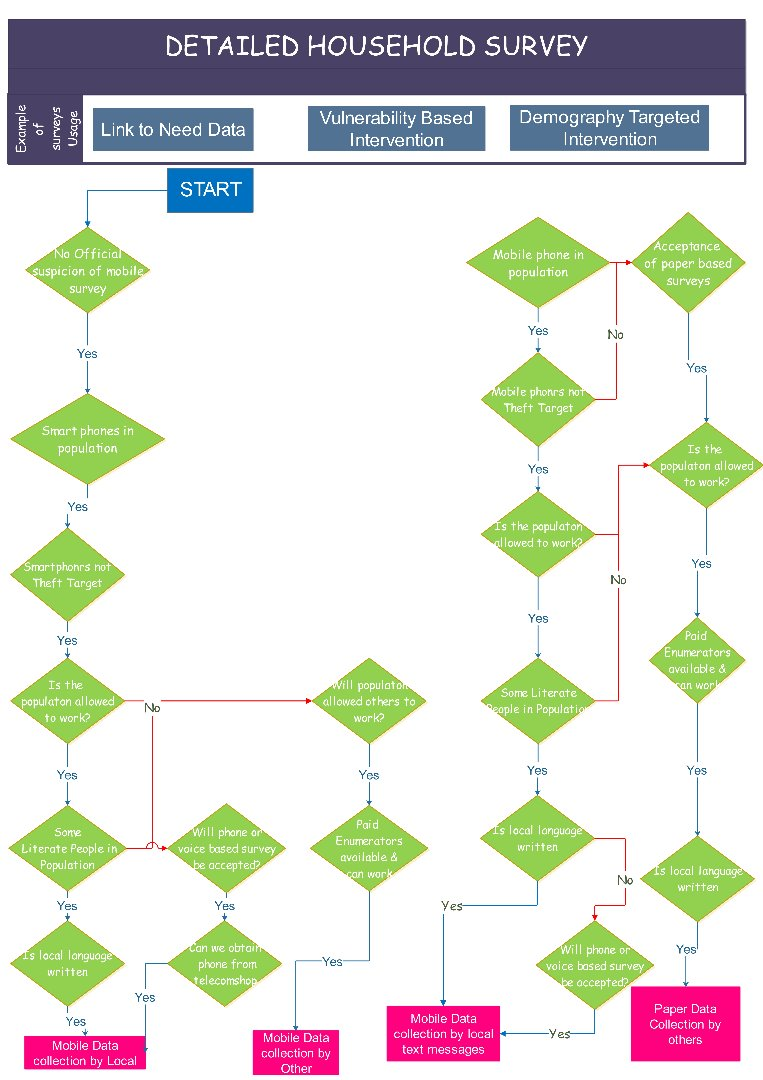
\includegraphics[width=0.9\textwidth]{images/Detailed_Household_Survey.jpeg}

\section{Tool Options}

\subsection{Aerial Mapping}

\subsubsection{Drones}

\subsubsection{Aircraft}

\subsubsection{Kites and balloons!}

\subsection{Mobile Data Collection}

\subsubsection{Community-Based Mobile Data Collection}
Mobile data collection is nothing new, however, in recent years it has become possible to use very low-educated people from within the beneficiary or local population, to gather data. 

\section{Recommendations}
MSF can take advantage of new opportunities. Not so much that there is new technology available---mobile data collection and drones have existed for some time now---but rather that both technologies have matured to the point that they can be used effectively in very low-resource settings.

\begin{itemize}
    \item MSF should consider using drones where rapid displacement has taken place in a setting that allows it without endangering the population or others (including MSF). Head counts are frequently dangerous and unpleasant exercises, and making use of newly available high-tech options---where ethical, appropriate and needed---is consistent with the duty of care to provide the best possible services to people.
    \item MSF should not consider mobile data collection to be the sole preserve of trained Community Health Care Workers or enumerators. Data collection can and should be seen as a collaboration and dialogue between the humanitarian community and the people we serve---use of local people, local devices, and open knowledge can greatly facilitate this. 
    
\end{itemize}

\end{document}
